\DeclareSong{Home}{Radical Face}{OnDa Drops Vol. 1: Do You Know They Way To Blue?}[3]
\vskip -1em
\intro{C\pause F\rep{4}}
\begin{strophe*}
  The \chord[c]{C}blood runs down my \chord[c]{F}legs \hfill
  I'm \chord[c]{Am}soaked through and \chord[c]{G}through but I'm in\chord[c]{F}different
  
  And there's \chord[c]{C}thunder in my \chord[c]{F}head \hfill
  I \chord[c]{Am}can't hear a \chord[c]{G}thing but it makes no \chord[c]{F}difference
  
  'cause \chord[c]{E\musf}now the \chord[c]{F}empire will \chord[c]{C}fall \hfill
  And \chord[c]{E\musf}we'll be \chord[c]{F}blamed for it \chord[c]{C}all
  
  And I wouldn't have it any other way\chord[c]{\null}
\end{strophe*}
\interlude{C\pause F\pause Am\pause G\pause F\pause G\rep{2}\Pause C}
\begin{strophe*}
  The \chord[c]{C}house went up in \chord[c]{F}flames \hfill
  And \chord[c]{Am}I sat and \chord[c]{G}watched you from a \chord[c]{F}distance
  
  The \chord[c]{C}wood creaked in com\chord[c]{F}plaint \hfill
  And the \chord[c]{Am}walls folded \chord[c]{G}in and took her \chord[c]{F}with them
  
  And \chord[c]{E\musf}now the \chord[c]{F}empire will \chord[c]{C}fall \hfill
  And \chord[c]{E\musf}we'll be \chord[c]{F}blamed for it \chord[c]{C}all
  
  And I wouldn't have it any other way\chord[c]{\null}
\end{strophe*}
\interlude{C\pause F\pause Am\pause G\pause F\pause G\rep{2}\Pause C}
\begin{strophe*}
  \chord[c]{C}Lost along the \chord[c]{E}way \hfill
  Quiet \chord[c]{Am}nights, grassy \chord[c]{G}roads, abandoned \chord[c]{F}homes
  
  And the \chord[c]{G}smell of \chord[c]{C}bones \hfill
  But I don't \chord[c]{E}mind
  
  As long as \chord[c]{Am}you are a\chord[c]{G}long for the \chord[c]{F}ride
\end{strophe*}
\vskip 1em
\begin{chorus*}
  Because you \chord[c]{G}feel like \chord[c]{C}home \hfill
  'cause you \chord[c]{G}feel like \chord[c]{F}home \rep{2}
  
  Because you \chord[c]{G}feel like \chord[c]{C}home
\end{chorus*}
\vskip 1em
\begin{strophe*}
  Abandoned \chord[c]{E}sky \hfill
  A flock of \chord[c]{Am}birds, some scattered \chord[c]{G}clouds and not a \chord[c]{F}wind
  
  And the \chord[c]{G}sounds of \chord[c]{C}light\hfill
  Down in these \chord[c]{E}fields
  
  We don't have \chord[c]{Am}much beyond the \chord[c]{G}clothes on our \chord[c]{F}backs
\end{strophe*}
\pagebreak
\begin{chorus*}
  But it \chord[c]{G}feels like \chord[c]{C}home \hfill
  But it \chord[c]{G}feels like \chord[c]{F}home \rep{2}
  
  But it \chord[c]{G}feels like\dots
\end{chorus*}
\vskip 1em
\begin{strophe*}
  \chord[c]{C}All the drafts, another \chord[c]{F}train has crashed, the smoke runs \chord[c]{G}from its \chord[c]{C}sides
  
  And I just pushed the re\chord[c]{F}mains aside and the pile's a \chord[c]{G}mile \chord[c]{Am}high
  
  I might \chord[c]{G}lose these hands, there's \chord[c]{F}never a guaran\chord[c]{C}tee\Pause\chord[c]{Am}
  
  And if I \chord[c]{G}fall to pieces \chord[c]{F}I would like to choose where I will land\pause\chord[c]{C}
\end{strophe*}

\vfill
\begin{center}
 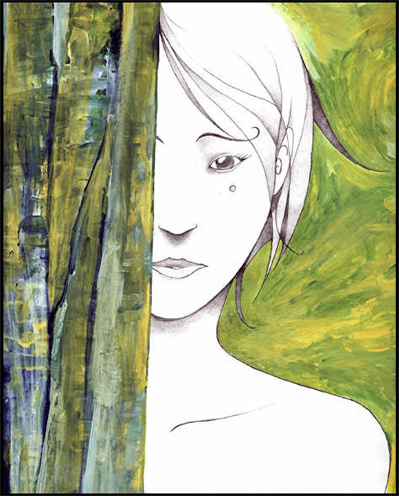
\includegraphics[scale=3]{pni35.jpg}
\end{center}
\vfill